% !TEX root = arbeit.tex
\section{Setup}\label{sec:setup}
	
	% Explain the 2 models and the differences.
	% Explain the part about the detector in a bit more details thus there are the most design improvements done so far.
	% Make a separate detector chapter? Explain the Setup and everything in that subchapter? Or just make one big chapter?

	% In case of a manual:
	% Chapter 1: NIM instrument description
	% Chapter 2: Manual (if it is not part of the Appendix)
	This chapter explains the NIM prototype and the NIM PFM model. It describes the differences between the two models. Special focus lay hereby on the design of the detector because there were done some major design improvements.
	
	
	\subsection{NIM Sensor Models \notes{Draft}}\label{subsec:setupInst}
	In this chapter, the NIM Prototype and the design of the NIM ProtoFlight Model (PFM) are described. The Prototype was build by Stefan Meyer and he also designed the NIM PFM \cite{Diss_Meyer}. The tests in Chapter \ref{sec:Exp} start with the configuration of the instruments as they are stated in this chapter.\\
	Fig.\ref{fig:SetupProtoISSim} shows the SIMION model of the Prototype ion-source Fig.\ref{fig:SetupPFMISSim} shows the ion-source of the PFM and Fig.\ref{fig:SetupFilElSim} shows the filament housing of the Prototype (left) and of the PFM (right). The PFM has seven electrodes less then the prototype to simplify the source. Manly LV electrodes were taken together (IS 1\& 2, IS 3 \& 4, IS 6 \& 7). IS 10 was removed and IS 11 was shifted towards the ionisation region. In the filament housing the filament electron repelling electrodes Fil 2-5 were taken together to one single repeller electrode Fil 2. The repeller electrode was splitted in 4 to compensate the filament position in case the filament was badly adjusted. For the PFM, the mounting of the filament holder was improved, therefore these 4 electrodes could be taken together to one single electrode.\\
	Fig.\ref{fig:SetupProtoReflSim} shows a schematics of the ion-mirror. The prototype ion-mirror consists of 14 ring-electrodes (R2-R15). R1 is the drift tube. Between the electrodes R4-R15 are resistors to connect the electrodes with each other to generate a linear voltage gradient when a voltage is applied at electrode R4 and R15. In addition, a voltage can be applied on electrode R8 allowing additional focusing of the ions in the ion-mirror.	The flight ion-mirror consists of a ceramic tube with two resistance spirals on its inner walls replacing electrodes R5-R7 and R9-R14. From the electrical point of view, the two ion-mirrors behave the same.
	
	% Detector: Anode, resistor, anode is floating on MCP front. May show a simple electrical schematics of how this work.
	% Schematic of the whole instrument, where every electrode is named, zoom in the filament and the detector section to describe, which electrode does what there. Very short description about their funcitonallity. Make the description in one model and highlight the differences between the Prototype and the PFM. May show the zoom of both models at the same time to show the difference of the two models.
	
	% State that for the tests at the CASYMIR test facility, the top cover of the antechamber was exchanged through one with one entrance hole at position +90°.
	
	% Fig.\ref{fig:SetupProtoISSim}-\ref{fig:} show the SIMION models of the Prototype ion-source, the filament housing, the ion-mirror and the detector. Fig.\ref{fig:SetupProto} shows the NIM Prototype as it was at the beginning of the measurement campaigns. Detailed cable schema and connection to the laboratory power supplies can be found in \cite{Diss_Meyer} Chap. 4.2.

		
		\begin{figure}[h] % Bild durch Bild mit Markierungen ersetzen
			\centering
			\includegraphics[width= 0.9\textwidth]{Setup/Proto_IS_sim.png}
			\caption{SIMION Model of the Ion-Source of the NIM Prototype \cite{Diss_Meyer}.}
			\label{fig:SetupProtoISSim}
		\end{figure}
		
		\begin{figure}[h] % Bild ersetzen. Evt noch Markierungen einfügen. IS bei den Nr. evt. noch einfügen.
			\centering
			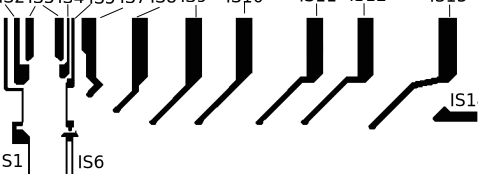
\includegraphics[width=0.9\textwidth]{Setup/ISFlight_bearb.png}
			\caption{SIMION Model of the Ion-Source of the NIM ProtoFlight Model.}
			\label{fig:SetupPFMISSim}
		\end{figure}
		\begin{figure}[h] % In Bild noch Fil 7/ Fil 4 durch IS5/ IS3 ersetzen.
			\begin{subfigure}{0.5\textwidth}
				\centering
				\includegraphics[width =0.85\textwidth]{Setup/Proto_FilEl_sim.jpg}
			\end{subfigure}
			\begin{subfigure}{0.5\textwidth}
				\centering
				\includegraphics[width = 0.85\textwidth]{Setup/PFM_FilEl_sim.jpg}
			\end{subfigure}
			\caption{Left: Prototype filament housing. Right: PFM filament housing.}
			\label{fig:SetupFilElSim}
		\end{figure}

		\begin{figure}[h]
			\centering
			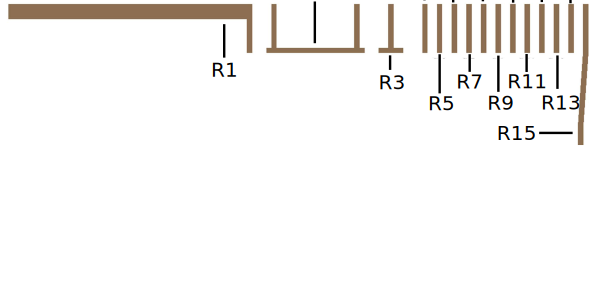
\includegraphics[width=0.9\textwidth]{Setup/Prototype_Reflectron_sim.png}
			\caption{SIMION Model of the ion-mirror of the NIM Prototype \cite{Diss_Meyer}.}
			\label{fig:SetupProtoReflSim}
		\end{figure}
		
		\begin{figure}[h] % Exchange reflectron through ion-mirror
			\centering
			\includegraphics[width=\textwidth]{Setup/Prototype_totPic.jpg}
			\caption{NIM Prototype \cite{Diss_Meyer}.}
			\label{fig:SetupProto}
		\end{figure}
		
		\begin{figure}[h] % Exchange picture through a picture collection (EGU2020 slid of the sensor in different states) Add a picture, where the inner parts are visible for comparison. Include a lineal ruler into the pictures.
			\centering
			\includegraphics[width=0.8\textwidth]{Setup/PFM_in_calib_Setup.JPG}
			\caption{NIM PFM sensor head in calibration setup.}
			\label{fig:SetupPFM}
		\end{figure}
		
			
%---------------------------------------------------------------------------------------------------------------

		\subsection{Detector design improvements}\label{subsubsec:SetFacPumpst} % May merge that chapter with the previous one.
		% Summary
		The detector suffered repeatedly discharges causing a failure of the diode, which is one of the key components of the detector (Fig.\,\notes{Ref. to the schema}). This lead to a redesign of the detector housing and to an exchange of the diode through a resistor, because the resistor is more robust concerning discharges.
		The discharges could be eliminated by a redesign of the detector housing.
		Fig.bla left shows an earlier version of the detector housing and Fig. bla right shows the design of the current flight detector.
		% Detailed explanation of how the detector actually works.
		Basically, the MCPs lay on a border about 1 mm above the anode. % Check distance
		A diode generates an additional voltage difference between the MCP backside and the anode to accelerate the electrons from the MCP backside towards the anode. Between this border and the MCP is the contact lug which is connected to the high voltage rail. On top of the upper MCP is the contact lug to connected to the corresponding voltage rail. On top of that is a bushing and a sort of screw. When tightening the screw, the bushing presses uniformly on the MCPs. In the old design, the thread for the screw was cut down to the boarder on which the MCPs lay. When assembling the whole stack, the MCPs often cant in the thread. Another challenge lay in tightening of the screw. When the screw was too loose, the top and the bottom contact lug had no reliable contact to the MCPs. When applying a high voltage over the whole MCP stack, the gap acts as an additional resistor over which the voltage build up resulting in a discharge between the corresponding electrode and the MCP. The discharge can propagate through the whole MCP stack and damage the diode and the capacitors. When the screw was tighten too much, the MCPs broke as they consist of lead glass and are very delicate in the mechanical point of view. As a consequence, the screw thread was cut less deep down and an additional boarder was made on which the bushing was pressed by the screw to make the assembly of the detector easier. In addition, the diode was exchanged through a resistor because the resistor is more robust in regards to the discharges. Due to the uncertainty in the manufacturing process of the detector housing, spacer rings are added between the bushing and the MCP to really close the gap. Due to that uncertainty, the number of rings needed for each detector has to be determined by trial.\\
		With the new design the detector suffered less discharges but as describe, the design is still not perfect. Therefore we decided to stay with the solution with the resistor instead of the diode.
		
		% Mechanical design, design improvements, electrical design and improvements (resistor, diode).
		% End with the calibration of U_{stack} vs. U_{MCP}
		
		
		% Also mention something about the design of the Prototype as a side note? Too big -> flexprint needed. miniaturization.
		% Mention something about that there are basically two different detector designs for the PFM detector from the electrical point of view and that that required an adaption of the setup to be able to calculate the voltage over the MCPs because the MCP Gain depends on the MCP voltage according to equation \notes{ref}.
		
		% Mechanical design improvement with the conclusion that the design is not perfect and therefore the desicion was to stay with the resistor instead of the diode. To calculate the MCP voltage, the lab measuring equipment had to be improved. With the flight electronics it is not possible to determine the current flowing through the MCPs an thus the MCP voltage. Therefore, a useful calibration is needed -> calculation with lab equipment. Differnt subchapter or put all in one as with the pulser discussion? Make it clear in the intro to the chapter...
		
		\subsection{MCP Voltage Calculation}\label{subsec:MCPVoltCalc} % If possible merge it with the previous chapter. Left it if it is easier to search about that calculation in a separate subchapter.
		
		The following section describes the design improvements of the PFM detector.
		
		
		
		
		Pumpstand nr. 2 was used to perform stand-alone tests with the different NIM detectors. The test setup consists of a vacuum chamber, a HV power supply, an oscilloscope, a computer to remote control the oscilloscope and a HV meter (Fig. \ref{fig:Pumpstand2}).\\
		
		During the further development of the detector, the diode in the detector was replaced by a resistor. To compare different measurements with each other it was required to determine the current flowing through the detector to determine the voltage over the MCPs.
		There are two different designs of the detector. One with a diode and one with a resistor
		
		Fig.\,\ref{fig:FlighElecSchema} shows the circuit diagram of the detector connected to an external power supply. Table\,\ref{tab:ElecSchemaVariableList} summarizes the used variables and gives a brief explanation.
		
		The aim is to calculate the voltage over the MCPs $U_{MCP}$ as a function of the voltage difference $U_{PSMCP}$ between the two outputs of the power supply $U_{PSA}$ (anode output of the power supply for the detector) and $U_{PSD}$ (MCP front voltage output of the power supply for the detector) as by the flight electronics the voltage $U_{PSMCP}$ and the drift voltage $U_{PSD}$ can be set.\\
		\begin{equation}
			U_{PSMCP} = U_{PSA} - U_{PSD}
			\label{eq:Upsmcp}
		\end{equation} % Phi_PSD is a negative voltage
		The MCPs have a voltage depended resistance which implies that we need the current $I_{MCP}$ flowing through the circuit to calculate $U_{MCP}$. As with the flight electronics it is not possible to measure this current, we do a calibration of the detector with laboratory electronics. This calibration is only valid when the detector does not come into saturation i.e. the current $I_A$ is low compared to the current $I_{RD}$ or the particle rate is below $10^6$ particles/sec.\\ % Ref. Stefan or someone else. How low? Particle rate lower than 10^6/sec -> current.
		$I_{MCP}$ is calculated by measuring the voltage over the test resistor $R_M$. $U_A$ is measured with a high voltage meter. By substituting $U_{PSA}$ with Eq.\eqref{eq:Upsmcp}, $I_{MCP}$ is then:
		\begin{equation}
			I_{MCP} = \frac{U_{PSMCP} + U_{PSD}-U_A}{R_M}
		\end{equation}
		The voltage $U_{PSMCP}$ can be written as:
		\begin{equation}
			U_{PSMCP} = U_{RM} + 2\cdot U_{Ri} + U_{RD} + U_{MCP}
			\label{eq:UpsmcpTot}
		\end{equation}
		With $U_{Ri} = I_{MCP}\cdot R_i$ the voltage over the input resistors $R_i$, which are there to damp noise coupled into the detector circuit from the power supply. In the final tests it is about 100 \si{\kilo\ohm}. $U_{RD}$ is the voltage over the diode replacement resistor $R_D$. Further explanation about the improvement of the detector can be found in chapter bla % Further comments about the developement needed.
		If the ion current $I_{ion}$ is low, this results in a low anode current $I_A$:
		\begin{equation}
			I_A = G\cdot I_{ion}
		\end{equation}
		with $G$ the MCP gain. % Order of magnitude?
		In this case $I_{MCP} = I_{RD}$ and:
		\begin{equation}
			U_{RD} = I_{MCP}\cdot R_D
		\end{equation}
		Solving Eq. \eqref{eq:UpsmcpTot} to $U_{MCP}$ results in:
		\begin{align}
			U_{MCP} =& U_{PSMCP} - U_{RM} - 2\cdot U_{Ri} - U_{RD}\\
			=& U_{PSMCP} - U_{PSMCP} + U_{PSD} - U_A - 2\cdot I_{MCP} R_i - I_{MCP} R_D\\
			=& (U_A - U_{PSD})\cdot(1 + \frac{2R_i + R_D}{R_M}) - U_{PSMCP}\frac{2R_i + R_D}{R_M}
		\end{align}
		
		
		\begin{figure}[h]
			\begin{subfigure}{.5\textwidth}
				\centering
				\includegraphics[width=0.8\textwidth]{Bilder/Galerie_Setup/Pumpstand2_midres.png}
			\end{subfigure}
			\begin{subfigure}{.5\textwidth}
				\centering
				\includegraphics[width=\textwidth]{Bilder/Galerie_Setup/Pumpstand_PSOszi.png}
			\end{subfigure}
			\caption{Left: Pumpstand nr. 2. Right: Power supply, oscilloscope and control computer for the stand-alone tests of the detector. The signal on the oscilloscope is a noise signal.}
			\label{fig:Pumpstand2}
		\end{figure}
		
		\begin{figure}[h]
			\centering
			\includegraphics[width = .8\textwidth]{Bilder/Detector_elec_schema.png}
			\caption{Electrical schematics of the NIM flight detector.}
			\label{fig:FlighElecSchema}
		\end{figure}
		
		
		\begin{table}[h]
			\begin{center}
			\begin{tabular}{|m{1.5cm}|m{5.4cm}|m{1.5cm}|m{5.4cm}|}
				\hline
				R\textsubscript{D}& Resistor replacing the former diode & U\textsubscript{A}& Voltage on the detector anode \\
				R\textsubscript{i} & Detector input resistor & U\textsubscript{MCP}& Voltage over the MCPs \\
				R\textsubscript{M}& Resistor used to determine I\textsubscript{MCP} &U\textsubscript{PSA} & Anode voltage output of power supply \\
				R\textsubscript{MCP}& MCP resistance & U\textsubscript{PSD} & Drift voltage output of power supply \\
				R\textsubscript{T} & 50\,$\Omega$ termination & U\textsubscript{PSMCP} & Voltage difference  between U\textsubscript{PSA} and U\textsubscript{PSD} \\
				I\textsubscript{A} & Current induced in the MCPs when an ion hits the MCPs & U\textsubscript{RD}& Voltage over R\textsubscript{D} \\
				I\textsubscript{ion} & Ion current hitting the MCPs & U\textsubscript{Ri}& Voltage over R\textsubscript{i} \\
				I\textsubscript{MCP} & Current flowing through the MCPs &U\textsubscript{RM}& Voltage over test resistor R\textsubscript{M}\\
				I\textsubscript{RD} & Current flowing through R\textsubscript{D} &&\\
				\hline
			\end{tabular}
			\end{center}
			\caption{Variable list for the detector.}
			\label{tab:ElecSchemaVariableList}
		\end{table}
	

		\begin{comment}
		\begin{table}
		\begin{tabular} {l | r | l}
			\hline
			Variable & Value & Description\\
			\hline
			U\textsubscript{PSD} & -2500 V & Drift voltage at the output of the power supply\\ % useless maybe
			U\textsubscript{PSMCP} & variable & Voltage difference between the two output channels of the power supply (phi)\\
			U\textsubscript{A} & variable & Detector anode voltage at the input\\
			$\varphi_{PSD}$ & -2500 V & Potential of the drift voltage at the output of the power supply\\
			$\varphi_{PSA}$ & variable & Potential of the anode at the outp of the power supply\\
			R\textsubscript{t} & 50 \si{\ohm} & terminating resistor\\
			R\textsubscript{A} & variable & equivalent resistance between MCP output and anode.\\
			R\textsubscript{i} & 100 \si{k\ohm} & Detector input resistance to damp noise coupled into the system by the super supply voltage line.\\
			I\textsubscript{A} & variable & Signal current produced by an ion triggering an electron avalanche in the MCPs\\
			\hline
		\end{tabular}
		\caption{Detector variables.}\label{tab:detVar}
		\end{table}
		\end{comment}
		
	
		%\includepdf[pages=-]{Setup/NIM_schema.pdf}
		\begin{figure}[h!]
			\centering
			\includegraphics[width= 0.95\textwidth]{Setup/NIM_schema.pdf}
			\caption{Schematics of NIM flight design with all electrodes marked in red.}
			\label{fig:MINPFMTot}
		\end{figure}
	
	
	
